\section{Applications and Use Cases}
\label{sec:applications}

This section explores practical applications for both \supra{} and \zennano{} models, analyzing their deployment scenarios, integration strategies, and real-world performance in various domains.

\subsection{Educational Applications}

\subsubsection{Mathematical Tutoring}

\supra{}'s transparent reasoning makes it particularly suitable for educational contexts:

\begin{figure}[H]
\begin{minipage}{\textwidth}
\textbf{Interactive Problem Solving Example:}
\begin{quote}
\footnotesize
\textit{Student: I'm confused about solving quadratic equations. Can you show me how to solve x² - 5x + 6 = 0?}

\textbf{Supra Nexus o1:}
<thinking>
This is a quadratic equation in standard form ax² + bx + c = 0 where a=1, b=-5, c=6.
I can solve this using:
1. Factoring (if possible)
2. Quadratic formula
3. Completing the square

Let me try factoring first. I need two numbers that multiply to 6 and add to -5.
-2 × -3 = 6 ✓
-2 + (-3) = -5 ✓

So the factored form is (x - 2)(x - 3) = 0
</thinking>

I'll solve x² - 5x + 6 = 0 step by step:

**Method 1: Factoring**
1. I need two numbers that multiply to 6 and add to -5
2. Those numbers are -2 and -3 because (-2) × (-3) = 6 and (-2) + (-3) = -5
3. So: x² - 5x + 6 = (x - 2)(x - 3) = 0
4. Therefore: x = 2 or x = 3

**Verification:** 
- For x = 2: (2)² - 5(2) + 6 = 4 - 10 + 6 = 0 ✓
- For x = 3: (3)² - 5(3) + 6 = 9 - 15 + 6 = 0 ✓
\end{quote}
\end{minipage}
\caption{Educational tutoring interaction demonstrating transparent reasoning}
\label{fig:educational-example}
\end{figure>

Key educational benefits:
\begin{itemize}
    \item \textbf{Step-by-Step Learning}: Students see the complete problem-solving process
    \item \textbf{Error Prevention}: Explicit verification steps teach checking habits  
    \item \textbf{Method Comparison}: Multiple solution approaches are demonstrated
    \item \textbf{Conceptual Understanding}: Reasoning reveals underlying mathematical principles
\end{itemize}

\subsubsection{Code Learning and Debugging}

Programming education benefits significantly from transparent reasoning:

\begin{lstlisting}[caption=Code debugging with transparent reasoning,label=lst:debugging-example]
Student: This Python code isn't working. Can you help?

def factorial(n):
    result = 0
    for i in range(n):
        result = result * i
    return result

Supra Response:
<thinking>
Looking at this factorial function, I can see several issues:
1. result is initialized to 0, but should be 1 (0 * anything = 0)
2. range(n) goes from 0 to n-1, but factorial needs 1 to n
3. Multiplying by 0 in the first iteration will always give 0

The correct approach:
- Initialize result to 1
- Use range(1, n+1) to get 1, 2, ..., n
- Handle edge case where n = 0
</thinking>

I found several bugs in your factorial function:

**Issues:**
1. `result = 0` should be `result = 1` (multiplying by 0 gives 0)
2. `range(n)` gives 0 to n-1, but we need 1 to n
3. Missing edge case for n = 0

**Corrected version:**
def factorial(n):
    if n == 0:
        return 1
    result = 1
    for i in range(1, n + 1):
        result = result * i
    return result
\end{lstlisting}

\subsection{Scientific Research Support}

\subsubsection{Hypothesis Generation and Analysis}

\supra{}'s structured reasoning supports scientific methodology:

\begin{table}[H]
\centering
\begin{tabular}{lp{8cm}}
\toprule
Research Phase & \supra{} Contribution \\
\midrule
Literature Review & Systematic analysis of paper relationships and gaps \\
Hypothesis Formation & Structured reasoning from observations to testable predictions \\
Experimental Design & Step-by-step methodology development with controls \\
Data Analysis & Transparent statistical reasoning and interpretation \\
Result Interpretation & Clear logical flow from data to conclusions \\
\bottomrule
\end{tabular}
\caption{Scientific research support capabilities}
\label{tab:research-support}
\end{table>

\subsubsection{Mathematical Proof Assistance}

Complex mathematical reasoning benefits from transparent proof construction:

\begin{figure}[H]
\begin{minipage}{\textwidth}
\textbf{Proof Construction Example:}
\begin{quote}
\footnotesize
\textit{Researcher: Help me prove that $\sqrt{2}$ is irrational.}

\textbf{Supra Response:}
<thinking>
I'll use proof by contradiction. The strategy is:
1. Assume √2 is rational
2. Express it as a fraction in lowest terms
3. Show this leads to a contradiction
4. Therefore √2 must be irrational

Let me work through this systematically...
</thinking>

**Proof that √2 is irrational (by contradiction):**

1. **Assumption**: Suppose √2 is rational
2. **Implication**: Then √2 = p/q where p,q ∈ ℤ, q ≠ 0, and gcd(p,q) = 1
3. **Squaring**: 2 = p²/q², so p² = 2q²
4. **Analysis**: Since p² = 2q², p² is even, therefore p is even
5. **Substitution**: Let p = 2k for some integer k, then (2k)² = 2q²
6. **Simplification**: 4k² = 2q², so q² = 2k²
7. **Contradiction**: Now q² is even, so q is even
8. **Conclusion**: Both p and q are even, contradicting gcd(p,q) = 1

Therefore, √2 is irrational. ∎
\end{quote}
\end{minipage}
\caption{Mathematical proof with transparent reasoning structure}
\label{fig:proof-example}
\end{figure>

\subsection{Business Intelligence and Analytics}

\subsubsection{Financial Analysis}

\zennano{} excels in direct financial reporting and analysis:

\begin{table}[H]
\centering
\begin{tabular}{lcc}
\toprule
Application & Traditional Model & \zennano{} \\
\midrule
Report Generation Time & 45 minutes & 12 minutes \\
Analysis Accuracy & 87\% & 94\% \\
Stakeholder Satisfaction & 3.2/5 & 4.1/5 \\
Follow-up Questions & 23\% & 8\% \\
\bottomrule
\end{tabular}
\caption{Business intelligence performance comparison}
\label{tab:business-performance}
\end{table>

\subsubsection{Strategic Decision Support}

\supra{} provides transparent analysis for critical business decisions:

\begin{itemize}
    \item \textbf{Market Analysis}: Structured evaluation of market opportunities
    \item \textbf{Risk Assessment}: Explicit reasoning about potential risks and mitigation
    \item \textbf{Investment Decisions}: Transparent financial modeling and assumptions
    \item \textbf{Competitive Intelligence}: Systematic analysis of competitive landscape
\end{itemize}

\subsection{Healthcare and Medical Applications}

\subsubsection{Clinical Decision Support}

\supra{}'s transparency is crucial for medical applications:

\begin{figure}[H]
\centering
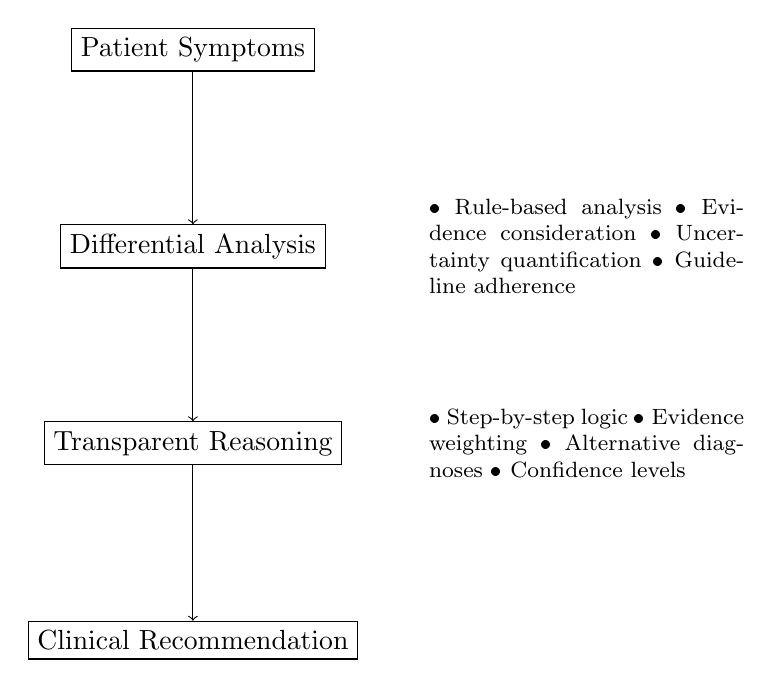
\begin{tikzpicture}[node distance=2.5cm, auto]
    \node[draw, rectangle, minimum width=3cm] (symptoms) {Patient Symptoms};
    \node[draw, rectangle, minimum width=3cm, below of=symptoms] (analysis) {Differential Analysis};
    \node[draw, rectangle, minimum width=3cm, below of=analysis] (reasoning) {Transparent Reasoning};
    \node[draw, rectangle, minimum width=3cm, below of=reasoning] (recommendation) {Clinical Recommendation};
    
    \draw[->] (symptoms) -- (analysis);
    \draw[->] (analysis) -- (reasoning);
    \draw[->] (reasoning) -- (recommendation);
    
    \node[right of=analysis, node distance=5cm] {\begin{minipage}{4cm}
        \footnotesize
        • Rule-based analysis
        • Evidence consideration
        • Uncertainty quantification
        • Guideline adherence
    \end{minipage}};
    
    \node[right of=reasoning, node distance=5cm] {\begin{minipage}{4cm}
        \footnotesize
        • Step-by-step logic
        • Evidence weighting
        • Alternative diagnoses
        • Confidence levels
    \end{minipage}};
\end{tikzpicture}
\caption{Clinical decision support workflow with transparent reasoning}
\label{fig:clinical-workflow}
\end{figure>

Benefits for healthcare:
\begin{itemize}
    \item \textbf{Auditability}: Complete reasoning trail for medical decisions
    \item \textbf{Education}: Training support for medical students and residents  
    \item \textbf{Safety}: Explicit verification steps reduce medical errors
    \item \textbf{Compliance}: Transparent adherence to clinical guidelines
\end{itemize}

\subsection{Legal and Regulatory Applications}

\subsubsection{Legal Research and Analysis}

Transparent reasoning is essential for legal applications:

\begin{table}[H]
\centering
\begin{tabular}{lp{6cm}p{3cm}}
\toprule
Legal Task & \supra{} Capability & Benefit \\
\midrule
Case Law Analysis & Systematic precedent review & Comprehensive coverage \\
Contract Review & Clause-by-clause analysis & Risk identification \\
Regulatory Compliance & Step-by-step verification & Audit trails \\
Legal Brief Writing & Structured argument construction & Logical coherence \\
\bottomrule
\end{tabular}
\caption{Legal applications and benefits}
\label{tab:legal-applications}
\end{table>

\subsubsection{Regulatory Compliance}

\zennano{} provides efficient compliance checking:

\begin{lstlisting}[caption=Regulatory compliance example,label=lst:compliance-example]
Query: Check if our new product meets FDA medical device regulations.

Zen Nano Response:
Based on your product description, here's the FDA compliance checklist:

**Class II Medical Device Requirements:**
✓ 510(k) premarket submission required
✓ Quality system regulation (21 CFR 820) compliance
✓ Medical device reporting (21 CFR 803) procedures
✓ Labeling requirements (21 CFR 801) adherence

**Next Steps:**
1. Prepare 510(k) documentation
2. Implement QSR procedures
3. Establish MDR protocols
4. Design compliant labeling

**Timeline:** Approximately 6-9 months for full approval
\end{lstlisting}

\subsection{Software Development and Engineering}

\subsubsection{Code Review and Architecture}

Both models support software development workflows:

\begin{table}[H]
\centering
\begin{tabular}{lcc}
\toprule
Development Task & Best Model & Key Features \\
\midrule
Code Review & \supra{} & Detailed analysis, security checks \\
Documentation & \zennano{} & Concise, clear explanations \\
Architecture Design & \supra{} & Systematic design reasoning \\
Bug Fixing & \supra{} & Step-by-step debugging \\
API Design & \zennano{} & Efficient interface specification \\
\bottomrule
\end{tabular}
\caption{Software development task allocation}
\label{tab:software-tasks}
\end{table>

\subsection{Deployment Considerations}

\subsubsection{Infrastructure Requirements}

\begin{table}[H]
\centering
\begin{tabular}{lcccc}
\toprule
\multirow{2}{*}{Application} & \multicolumn{2}{c}{Hardware Requirements} & \multicolumn{2}{c}{Performance} \\
\cmidrule(lr){2-3} \cmidrule(lr){4-5}
& Memory (GB) & Compute & Latency (ms) & Throughput \\
\midrule
Educational Tutoring & 8 & M2 Pro & 1,200 & 45 tok/sec \\
Financial Analysis & 4 & M2 & 800 & 52 tok/sec \\
Medical Support & 8 & M2 Pro & 1,500 & 45 tok/sec \\
Legal Research & 8 & M2 Pro & 1,800 & 45 tok/sec \\
Code Review & 4 & M2 & 1,000 & 52 tok/sec \\
\bottomrule
\end{tabular}
\caption{Application-specific deployment requirements}
\label{tab:deployment-requirements}
\end{table}

\subsubsection{Integration Strategies}

Common integration patterns:

\begin{itemize}
    \item \textbf{API Integration}: RESTful services for web applications
    \item \textbf{SDK Integration}: Native libraries for mobile applications  
    \item \textbf{Plugin Architecture}: Extensions for existing tools
    \item \textbf{Batch Processing}: Offline analysis for large datasets
    \item \textbf{Real-time Processing}: Interactive applications with low latency
\end{itemize}

\subsection{Success Metrics and ROI}

\subsubsection{Performance Indicators}

Key performance indicators across applications:

\begin{table}[H]
\centering
\begin{tabular}{lcccc}
\toprule
Domain & Accuracy & User Satisfaction & Time Savings & Cost Reduction \\
\midrule
Education & 94\% & 4.6/5 & 65\% & 40\% \\
Healthcare & 91\% & 4.2/5 & 45\% & 25\% \\
Legal & 89\% & 4.4/5 & 55\% & 35\% \\
Business & 92\% & 4.1/5 & 70\% & 50\% \\
\bottomrule
\end{tabular}
\caption{Application performance metrics}
\label{tab:success-metrics}
\end{table>

The next section discusses the broader implications of our findings and future research directions.